\section{Static Multiple-Issue Processor: Approccio VLIM }\label{capitolo4}
Fino ad ora abbiamo analizzato tecniche che permettono di estrapolare il parallelismo dalle istruzioni solo nel caso in cui queste siano prelevate dalla memoria in modo sequenziale una alla volta; con questo meccanismo abbiamo che il CPI massimo che possiamo ottenere è 1 ovvero possiamo eseguire, nel migliore dei casi, al massimo una istruzione per ciclo.\\
Introduciamo ora una categoria di processori che, invece, sono in grado di prelevare più di una istruzione per ogni ciclo di clock. Questi processori possono essere a \emph{scheduler dinamico} ovvero possono prelevare un numero diverso di istruzioni ad ogni ciclo di clock, oppure a scheduler statico che preleva un numero prefissato di istruzioni ad ogni ciclo.\\
Il numero di istruzioni che si possono prelevare ad ogni ciclo può variare da un minimo di 1 ad un massimo di 8 il CPI in questo caso diventa $CPI= 1/ \#istruzioni \ prelevate$. Questo tipo di processore viene definito \emph{processore superscalare}. Lo scheduler può essere implementato esclusivamente tramite lo hardware anche se il compilatore può migliorare notevolmente la qualità dello scheduler. Lo hardware risistema le istruzioni in esecuzione per ridurre il numero degli stalli mentre mantiene il flusso dei dati e il comportamento delle eccezioni, i vantaggi principali sono la possibilità di gestire casi di dipendenze sconosciute al tempo della compilazione, l'utilizzo di un compilatore semplificato ed infine la possibilità per il codice compilato di essere eseguito su pipeline diverse; questi vantaggi sono ottenuti al costo di una maggiore complessità dello hardware e di un maggiore consumo energetico.\\
Lo scheduler statico utilizza compilatori con algoritmi sofisticati per estrapolare ILP da codice sorgente e individuando quando due istruzioni possono essere eseguite in parallelo. Tuttavia il problema principale è che questa analisi può essere effettuata solo tra \emph{basic block}, ovvero tra piccoli segmenti di codice sequenziale privi di salti ad eccezione del punto iniziale e nessun salto in uscita se non alla fine. Tipicamente questi blocchi hanno una lunghezza compresa tra le 4 e le 7 istruzioni. Un altro fattore che limita la quantità di ILP che si può estrapolare dal codice è la dipendenza dei dati; il compilatore tuttavia può, in certa misura, eliminare alcune false dipendenze in modo da aumentare il parallelismo. Per aumentare notevolmente le performance dobbiamo estrapolare il parallelismo tra diversi basic block.\\
Come primo passo bisogna determinare le dipendenze tra le istruzioni in quanto queste dipendenze determinano il livello di parallelismo del programma. Come abbiamo visto esistono tre tipi di dipendenza:
\begin{itemize}
\item Dipendenza dei dati.
\item Dipendenza dei nomi (WAR e WAW)
\item Dipendenze di controllo
\end{itemize}
\subsection{Processori VLIW}
Come abbiamo visto la ricerca delle dipendenze tramite hardware e lo scheduling dinamico richiedono un grande consumo di area e di energia. L'idea generale è quella di ridurre questi due fattori spostando sul compilatore la decisione di quali operazioni possono essere eseguite in parallelo. Queste operazioni parallele sono raggruppate dal compilatore in un unico pacchetto chiamato \emph{bundle} così che l'hardware non debba controllare eventuali dipendenze.\\
Il compilatore deve essere certo che non vi siano dipendenze tra le istruzioni inserite nel bundle, tuttalpiù può indicare quando una dipendenza può presentarsi.\\
Il vantaggio di questo approccio è che si semplifica notevolmente l'hardware si ha un notevole risparmio sul consumo di energia e si ottengono buone performance grazie a ottimizzazioni del compilatore.\\
Un singolo pacchetto è in realtà un istruzione molto grande (64, 128 o più bits) nella quale sono inserite più operazioni. In principio i processori VLIW erano molto rigidi sul formato delle istruzioni e richiedevano la ricompilazione del programma nel caso di utilizzo su diversi tipi di hardware.\\
L'istruzione lunga è composta da una serie di campi chiamati \emph{slot} corrispondenti ognuno ad un'unità funzionale; ad esempio una \emph{5-issue VLIW} è un'istruzione lunga che contiene 5 operazioni ad esempio una operazione intera o di salto, due operazioni con la virgola e due operazioni di load/store. In questo modo la fase di decodifica si riduce alla decodifica di ogni istruzione come si può vedere nella \figurename\,\ref{fig:vliwarch}
\begin{figure}
\centering
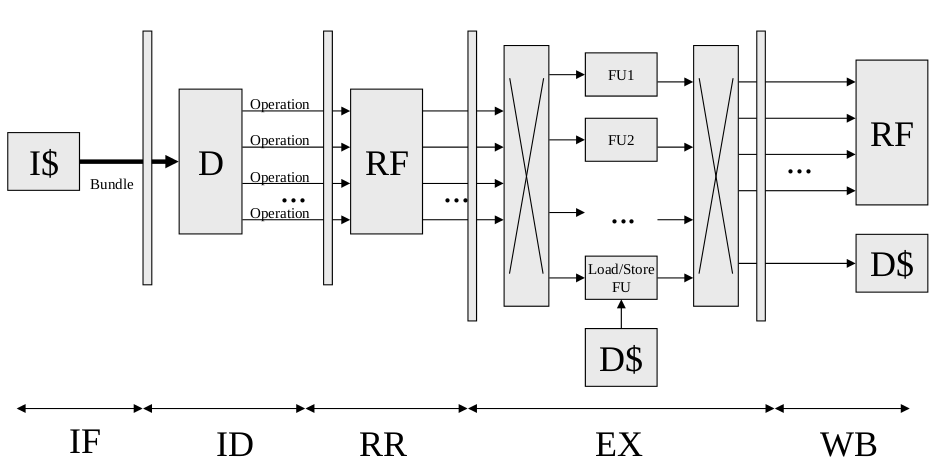
\includegraphics[scale=0.5]{img/vliwarch.png}
\caption{Architettura di una pipeline per VLIW}\label{fig:vliwarch}
\end{figure}
Sfortunatamente le operazioni VLIW non sono di tipo atomico, ovvero non avvengono in un solo ciclo di clock perciò la latenza delle operazioni deve essere nota al compilatore ad esempio:
\begin{verbatim}
I		[C=A*B, ...];
I+1		[nop,   ...];
I+2		[X=C*F, ...];
\end{verbatim}
In questo caso l'operazione "\*" ha una latenza di 2 perciò il compilatore inserisce una \texttt{nop} al secondo ciclo in quanto \emph{C} non è ancora pronta; se il compilatore schedulasse la seconda moltiplicazione nel secondo ciclo si comprometterebbe la corretta esecuzione del programma. Le dipendenze di tipo WAW e WAR sono risolte dal compilatore e non dallo hardware tenendo conto della latenza delle diverse FU. Per quanto riguarda, invece, le dipendenze di tipo RAW i processori superscalari inseriscono delle \texttt{nop} oppure eseguono se possibile, delle istruzioni successive. Nei processori VLIW  sono inserite dal compilatore durante la fase di scheduling, idealmente sono usate, se possibile, solo istruzioni non coinvolte in dipendenze, altrimenti sono generate delle \texttt{nop}. Tutte le dipendenze vengono risolte dal compilatore, il quale fornisce anche informazioni riguardo alle predizioni dei salti; l'unico tipo di dipendenza che rimane da risolvere sono quelle di controllo che viene evitata dallo hardware abortendo l'esecuzione delle operazioni in caso di predizione incorretta.\\
Un esempio di meccanismo VLIW è presentato in \figurename\,\ref{fig:VLIWexemp}
\begin{figure}[htb]
\centering
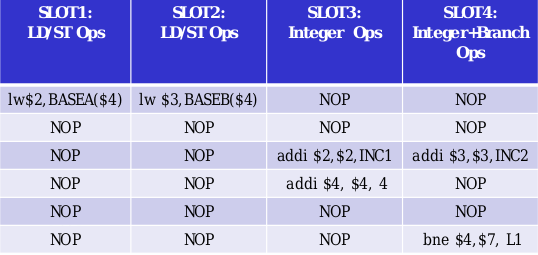
\includegraphics[scale=0.5]{img/vliwexemp.png}
\caption{Esempio di utilizzo di Very Long Instruction World con queste FU: 2 LD/ST, 1 Int e 1 Int/Branch}\label{fig:VLIWexemp}
\end{figure}
I vantaggi dell'utilizzo delle VLIW sono il fatto che il compilatore può analizzare il codice ad un livello più alto rispetto a quello che fa lo hardware, in questo modo, tramite sofisticati algoritmi, si può estrapolare un maggiore parallelismo tra le diverse istruzioni e quindi aumentare le performance. Inoltre, le istruzioni hanno dei campi prefissati è quindi più facile decodificarle. Infine, si riduce notevolmente la complessità dello hardware tramite una superficie minore e quindi un minor consumo di energia e la possibilità di introdurre più FU. Le difficoltà all'applicazione su larga scala di questo meccanismo sono la necessità di avere una tecnologia di compilazione che individui ed estrapoli il parallelismo anche oltre i singoli \emph{basic block}. Inoltre la dimensione del codice aumenta di molto a causa delle numerose \texttt{nop} che vengono introdotte; infine, la complessità del Register File e della circuiteria di trasporto verso le FU è incrementata di molto. L'aspetto più importante che però limita l'utilizzo della tecnologia VLIW è l'incompatibilità binaria, ad esempio architettura con lo stesso ISA ma diversi bundle VLIW sono incompatibili, ma anche architetture con lo stesso ISA e con lo stesso bundle ma latenze differenti sono incompatibili. L'unica soluzione a questo problema è la \emph{Just In Time Compilation} ma è molto costosa. Perciò, in molti casi, la VLIW è utilizzata solo nei sistemi embedded dove la compatibilità binaria non è un fattore rilevante.
\subsubsection{Alcuni esempi}
Analiziamo ora alcuni esempi dei più diffusi processori VLIW presenti in commercio.
\paragraph{STMicroelectronics ST200}
Processore embedded pensato per l'utilizzo e la gestione dei media; esso è un processore VLIW di tipo cluster con quattro cluster eseguiti con un singolo PC. Ogni cluster ha 4 slot e può eseguire perciò 4 istruzioni contemporaneamente, 1 salto, 1 load/store, due moltiplicazioni. Ogni cluster ha a disposizione un banco di 64 registri.
\paragraph{NXP Trimedia}
\upercase{é} un processore per i media con cinque unità di esecuzione tali unità richiedono 15 porte in lettura e 5 in scrittura, ogni unità necessità di tre porte in lettura per leggere i due operandi e un \emph{guard operand} il quale condiziona l'esecuzione di ogni operazione.
\paragraph{VLIW vs EPIC: Intel IA-64}
Un evoluzione del VLIW è stato EPIC (\emph{Explicitly Parallel Instruction Computer}) che al contrario del VLIW permette una flessibilità del formato delle istruzioni inoltre indica quando un istruzione non può essere eseguita in parallelo alle successive.\\
Una prima implementazione di questa tecnologia è stato \emph{Intel Itanium} il quale permetteva un alto parallelismo e una pipeline profonda con una frequenza di clock molto bassa 800MHz. Inoltre, aveva 128 registri a 64-bit per gli interi e 128 registri a 82 bit per i numeri con la virgola.\\
I registri di tipo integer sono configurati per aiutare ed accellerare le chiamate a procedura usando lo stack dei registri, questo meccanismo è simile a quello utilizzato nei RISC e nelle architetture SPARC. I registri dallo 0 al 31 sono sempre accessibili tramite il loro indirizzo reale, i registri 32-128 sono allocati come register stack ed ogni procedura ne può allocare alcuni (da 0 a 96) rinominando i registri fisici.\\
Un \emph{instructions group} è una sequenza di istruzioni consecutive senza dipendenze dei dati, queste istruzioni perciò possono essere eseguite in parallelo se sono disponibili le risorse hardware. La lunghezza dei gruppi è arbitraria ma il compilatore deve separare esplicitamente i due gruppi inserendo uno \emph{stop} tra due istruzioni che appartengono a due gruppi diversi. Nel IA-64 le istruzioni sono codificate in bundle di lunghezza 128 bit, ogni bundle è composto da un campo \emph{templete} di 5 bit e da 3 istruzioni di 41 bits.\\
Il processore Itanium ha una pipeline composta da 10 stadi come possiamo vedere in \figurename\,\ref{fig:itapipe}
\begin{figure}
\centering
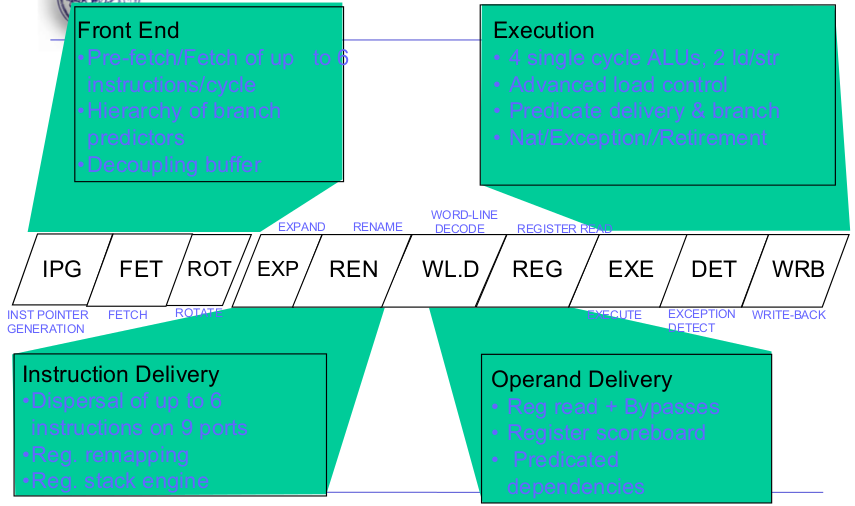
\includegraphics[scale=0.5]{img/itapipe.png}
\caption{Stage della pipeline di un processore Itanium}\label{fig:itapipe}
\end{figure}
Come vediamo dalla \figurename\,\ref{fig:itapipe} possiamo raggruppare i diversi stage in quattro gruppi:
\begin{description}
\item[Front-end:] composto dagli stage IPG, Fetch e Rotate, precaricano 32 byte per clock (2 bundle) in un buffer di precarico, il quale mantiene 24 istruzioni, in questa fase si possono effettuare delle predizioni tramote un predittore adattativo multilivello.
\item[Instruction delivery:] formato dagli stage EXP e REN i quali distribuiscono le istruzioni alle 9 unità funzionali ed effettuano il renaming dei registri.
\item[Operand delivered:] formato dagli stage WLD e REG, accede ai registri e verifica eventuali dipendenze.
\item[Execution:] composto dagli ultimi tre stage (EXE, DET e WRB) si occupa di eseguire le istruzioni individuando eventuali eccezioni ed inoltre effettua il write-back dei risultati.
\end{description}
\paragraph{Processore Crusoe}
Il processore Crusoe è un processore VLIW con esecuzione sequenziale formato da 64 registri di tipo integer e da 32 registri per i \emph{floating point}. Esso è formato da una pipeline a 6 stadi per gli integer: 2 fetch, 1 di decodifica, 1 register read, 1 execution e 1 write back; e da una pipeline a 10 stadi per le operazioni in virgola mobile, che comprendono 4 stadi supplementari per la fase di esecuzione.\\
I processori Crusoe hanno a disposizione 5 unità funzionali:
\begin{itemize}
\item ALU;
\item Compute che è un unità che può occuparsi di due ALU contemporaneamente o una floating point o un'operazione sui media.
\item Memory: che implementa le operazioni di load e di store.
\item Branch: per eseguire un istruzione di salto
\item Immediate:una istruzioni a 32 bit utilizzata immediatamente da un'altra operazione
\end{itemize}
\subsection{Code scheduling VLIW}
L'obiettivo principale dello scheduling nei processori VLIW è quello di stabilire staticamente l'ordine di esecuzione delle istruzioni nel codice oggetto in modo che queste vengano eseguite in modo corretto ed efficiente.\\
Il meccanismo base per schedulare le istruzioni in modo efficente è quello di dividere il codice in blocchi base a questo punto per ogni blocco base si costruisce un grafico delle dipendenze come quello mostrato in \figurename\,\ref{fig:depgra}
\begin{figure}[htb]
\centering
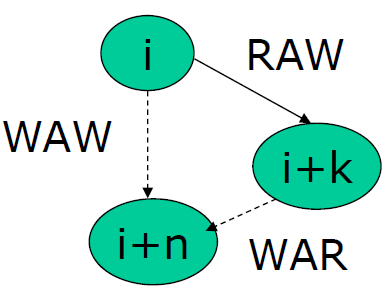
\includegraphics[scale=0.5]{img/depgrap.png}
\caption{Esempio di grafico delle dipendenze tra le istruzioni di un blocco base}\label{fig:depgrap}
\end{figure}
Un grafico delle dipendenze cattura tutti i tipi di dipendenze (WAR, WAW e RAW) le dipendenze WAR e WAW però sono dipendenze solo di nome in quanto sono dovute al riuso dei registri o delle variabili. Dal grafico delle dipendenze si può individuare il cosiddetto \emph{critcal path} ovvero il percorso più lungo in un grafico delle dipendenze; questo percorso determina il minimo tempo di esecuzione come possiamo vedere dalla \figurename\,\ref{fig:criticalpath}
\begin{figure}[htb]
\centering
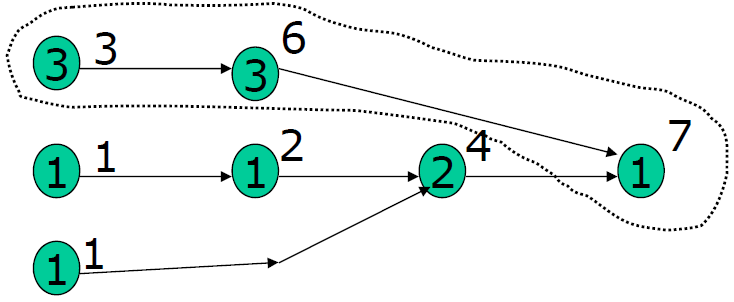
\includegraphics[scale=0.5]{img/criticalpath.png}
\caption{Esempio di \emph{critical path}}\label{fig:criticalpath}
\end{figure}
Dal quale si possono calcolare la lunghezza di ogni percorso tramite la formula
$$LP(i)= Max(LP(Pred(i))+Latency(i)$$
mentre il \emph{critical path} è dato dal valore massimo tra tutte le lunghezze
$$LCP= Max(LP(i))$$
Lo scheduler in teoria dovrebbe programmare l'esecuzione di ogni operazione del \emph{critical path} in modo da minimizzare il tempo di esecuzione e parallelamente schedulare le altre istruzioni, questo però è possibile soltanto nel caso di processori con risorse infinite. Con risorse finite invece il tempo di esecuzione dipende anche da come sono schedulate le rimanenti operazioni. Inoltre, uno scheduler ottimo analizza in modo esaustivo lo spazio degli schedule disponibili per minimizzare il tempo di esecuzione, ma tale analisi è un problema NP-completo siamo perciò costretti ad usare dei meccanismi euristici.
\subsection{List-based scheduling}
In questo tipo di scheduling per ogni ciclo di clock viene selezionata un'istruzione da un \emph{ready set} che può essere inserita in uno degli slot. Un'istruzione si definisce \emph{ready} quando tutti i suoi predecessori sono già stati schedulati e tutti gli operandi necessari sono disponibili. All'inizio dello scheduling tutte le operazioni all'inizio del grafico sono inserite nel \emph{ready set} e ad ogni ciclo si cerca di schedulare tutte le istruzioni nel set nel caso più istruzioni siano presenti si schedula quella con la priorità maggiore.\\
Per implementare questo meccanismo è necessario però tenere traccia di quali risorse sono occupate per fare questo si utilizza una \emph{Resource Reservation Table} ovvero una tabella che indica quali risorse sono occupate in un determinato istante di tempo.\\
Un esempio di tale sistema è mostrato in \figurname\,\ref{fig:reservation}
\begin{figure}[htb]
\centering
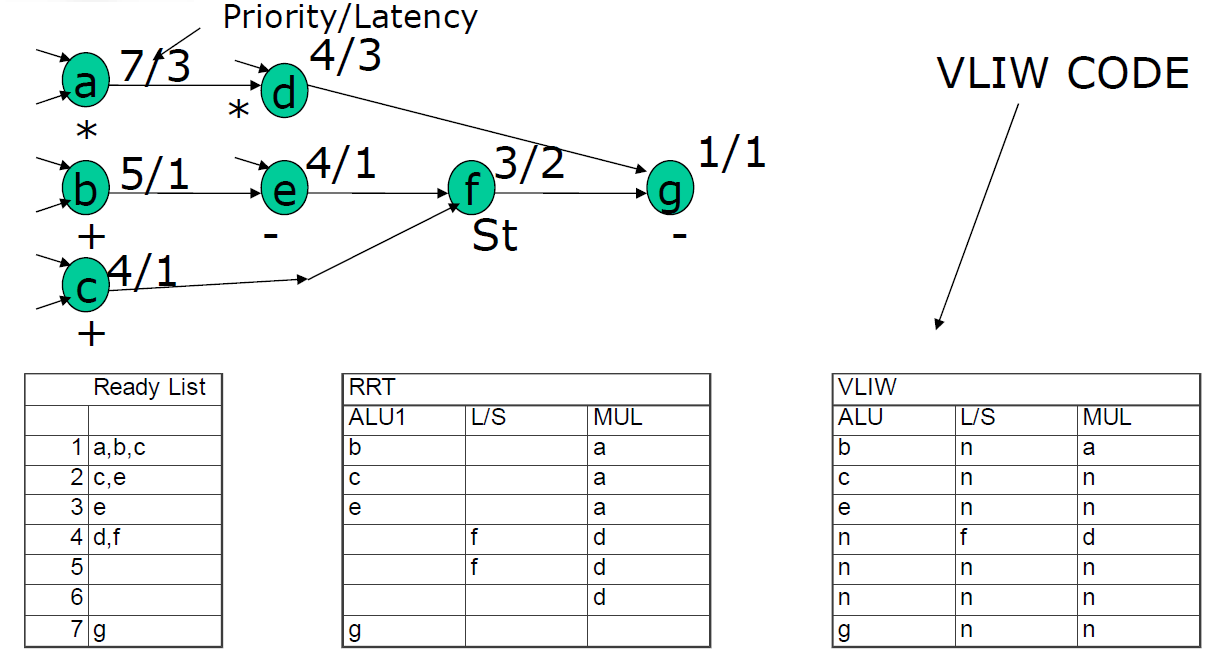
\includegraphics[scale=0.5]{img/reservation.png}
\caption{Esempio di scheduling List-Based con utilizzo di Reservation Table}\label{fig:reservation}
\end{figure}
\subsection{Global e Local scheduling}
Per esplorare tutto il possibile parallelismo presente è necessario che il compilatore espanda la dimensione del basic block o che scheduli parallelamente istruzioni che appartengono a basic block differenti.
Le tecniche di \emph{local scheduling}  operano su di un singolo basic block e possono essere tecniche di \emph{Loop Unrolling} o di \emph{Software Pipelining}.
Le tecniche di \emph{global scheduling} espandono la ricerca del parallelismo al di fuori del singolo basic block e alcune tecniche sono \emph{Trace Scheduling} e il \emph{Superblock Scheduling}.\\
\paragraph{Loop unrolling}
Il \emph{loop unrolling} è una tecnica di scheduling locale che permette al compilatore di incrementare la quantità di parallelismo disponibile in un basic block. Per fare ciò il compilatore replica il corpo di un loop diverse volte (dipende dal fattore di \emph{unrolling}) sistemando poi il codice di terminazione del ciclo. Per effettuare questa operazione però il compilatore deve prima testare l'indipendenza tra le diverse iterazioni.\\
Il \emph{loop unrolling} permette di incrementare il numero di operazioni effettuate ad ogni ciclo minimizzando però il numero di salti da effettuare; inoltre, aumentando il numero di operazioni si aumenta la lunghezza del blocco base permettendo al compilatore di effettuare uno scheduling più efficiente. Gli svantaggi di questa tecnica sono però l'aumento della dimensione del codice e il numero di registri richiesto per l'esecuzione.\\
Un esempio di loop unrolling è mostrato nelle \figurname\,\ref{fig:unroll1} e \figurname\,\ref{fig:unroll2} dove si mostra un unrolling di fattore di srotolamento di 2.
\begin{figure}[htb]
\centering
\subfigure[loop base]{
\label{fig:unroll1}
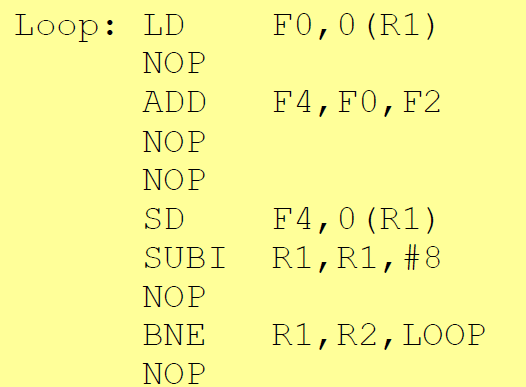
\includegraphics[scale=0.4]{img/unroll1.png}
}
\subfigure[loop unrolled]{
\label{fig:unroll2}
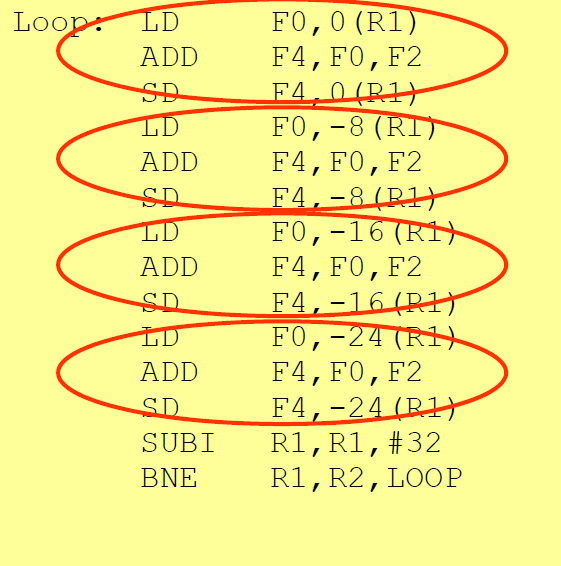
\includegraphics[scale=0.4]{img/unroll2.png}
}
\caption{Esempio di unrolling con fattore 2}
\end{figure}
\paragraph{Loop-carried dependences}
Il loop-carried è una tecnica incentrata sull'analisi delle dipendenze presenti tra gli operandi all'interno delle diverse interazioni di un loop. Si hanno delle dipendenze tra due interazioni di un loop quando un valore in una interazioni dipende da un secondo valore prodotto in una interazione precedente. Un esempio di questa dipendenza è dato dal seguente codice:
\begin{verbatim}
for (i = 6; i < 100; i++)
{
	Y[i] = Y[i-5] + Y[i];
}
\end{verbatim}
In questo caso ogni iterazione dipende dalla 5 iterazione precedente e quindi le iterazioni \texttt{i, i+1, i+2, i+3, i+4} sono indipendenti (\texttt{i+5} dipende dall'iterazione \texttt{i}). Trovando il fattore di indipendenza si può trovare effettuare un \emph{unrolling} del ciclo come segue:
\begin{verbatim}
for (i = 6; i < 100; i=i+5)
{
	Y[i] = Y[i-5] + Y[i];
	Y[i+1] = Y[i-4] + Y[i+1];
	Y[i+2] = Y[i-3] + Y[i+2];
	Y[i+3] = Y[i-2] + Y[i+3];
	Y[i+4] = Y[i-1] + Y[i+4];
}
\end{verbatim}
Si riesce così ad estendere il blocco base ma il fattore di \emph{unrolling} non può essere maggiore di 5.
\paragraph{Loop peeling e fusion}
La tecnica di \emph{peeling \& fusion} è una tecnica che consiste nell'eliminare (sbucciare) da un ciclo le interazioni "superflue" in modo da poterlo fondere con un secondo ciclo; ad esempio prendiamo in considerazione due cicli:
\begin{verbatim}
for (i = 0; i < 102; i++) b[i] = b[i-2] + c;
for (j = 0; j < 100; j++) a[j] = a[j] * 2;
\end{verbatim}
In questo caso "sbucciamo" il primo ciclo delle ultime due iterazioni e lo fondiamo poi con il secondo ciclo, otteniamo così:
\begin{verbatim}
for (i = 0; i < 100; i++)
{
	b[i] = b[i-2] + c;
	a[i] = a[i] * 2;
}
b[100] = b[98] + c;
b[101] = b[99] + c;
\end{verbatim}
dove abbiamo un ciclo che "fonde" i due precedenti e due operazioni aggiuntive che servono a compensare le due iterazioni mancanti del primo.
\paragraph{Software pipeline}
Supponiamo di avere un loop nel quale ad ogni iterazione possiamo identificare delle istruzioni indipendenti differenti come quello mostrato in \figurename\,\ref{fig:swpipe}
\begin{figure}[htb]
\centering
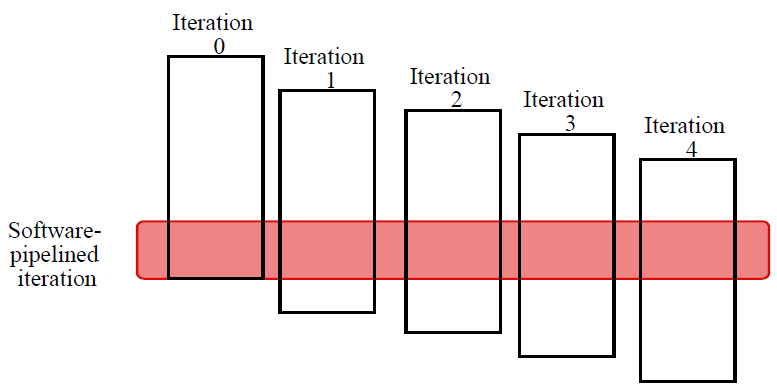
\includegraphics[scale=0.5]{img/swpipe.png}
\caption{Loop con istruzioni indipendenti ad ogni iterazione}\label{fig:swpipe}
\end{figure}
A questo punto possiamo riorganizzare queste istruzioni in un nuovo loop nel quale ad ogni iterazione si eseguano delle istruzioni provenienti da diverse iterazioni.
Questa tecnica può essere considerata un po come un \emph{symbolic loop unrolling}.\\
Prendiamo in esempio il seguente loop dove sono presenti delle dipendenze interne al loop.
\begin{verbatim}
for(i = 0; i < 100; i++)
{
	A[i] = B[i];
	A[i] = A[i]+1;
	C[i] = A[i];
}
\end{verbatim}
In \figurename\,\ref{fig:iteration} vediamo lo svolgimento delle diverse iterazioni; i riquadri nella figura indicano il nuovo ciclo che si viene a creare che viene mostrato in \figurename\,\ref{fig:newcicle}. Il vantaggio di questa tecnica è che consuma meno spazio del loop unrolling, in quanto non vi è la necessità di duplicare il codice. Si riempe e si svuota la pipe una volta sola per ogni loop al contrario del caso del loop unrolling che si riempe e si svuota ad ogni interazione. Infine tale tecnica può essere associata anche al loop unrolling per incrementarne le prestazioni.
\begin{figure}[htb]
\centering
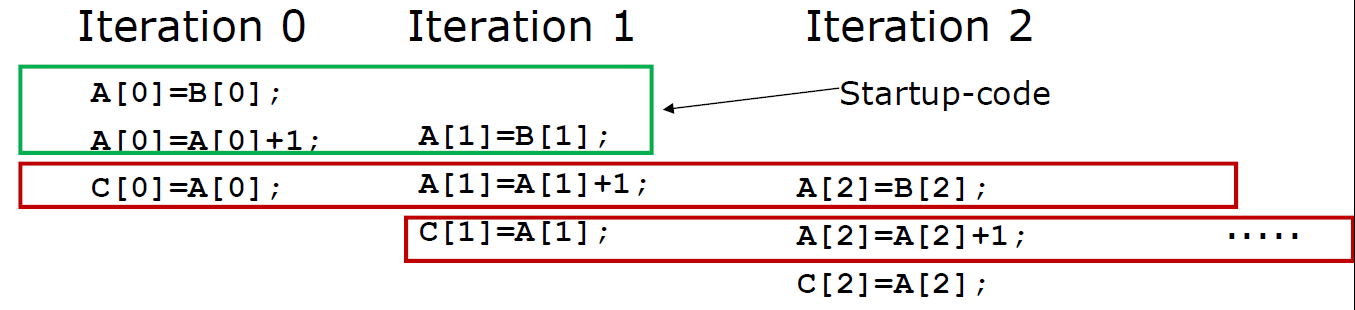
\includegraphics[scale=0.5]{img/iteration.png}
\caption{Svolgimento delle diverse iterazioni}\label{fig:iterazioni}
\end{figure}
\begin{figure}[htb]
\centering
\includegraphics[scale=0.5]{img/newcile.png}
\caption{Nuovo codice che implementa il loop}\label{fig:newcile}
\end{figure}
\paragraph{Trace scheduling}
I sistemi di local scheduling funzionano solo quando i loop contengono un singolo basic block, quando i corpi dei loop contengono dei flussi di controllo allora è necessario espandere lo scheduling attraverso i diversi basic block tramite tecniche di \emph{global schedulig}.\\
Il \emph{trace scheduling} è la prima tecnica che analizzeremo e consiste nel tentare di trovare del parallelismo attraverso i salti condizionati. Si compone di due passi, il primo consiste nel trovare una sequenza di blocchi base composta dalla più lunga sequenza di istruzioni, la seconda fase consiste nel compattare questa sequenza in poche istruzioni VILW inserendo delle istruzioni di compensazione in caso di predizione errata. Questa tecnica è una forma di speculazione del compilatore.
\paragraph{Superblock scheduling}
Questa è una tecnica di ottimizzazione del \emph{trace scheduling} che consiste nel creare un \emph{superblocco} formato da diversi blocchi base con un unico punto d'entrata e molteplici flussi di controllo in uscita come mostrato in \figurename\,\ref{fig:superblock}.
\begin{figure}[htb]
\centering
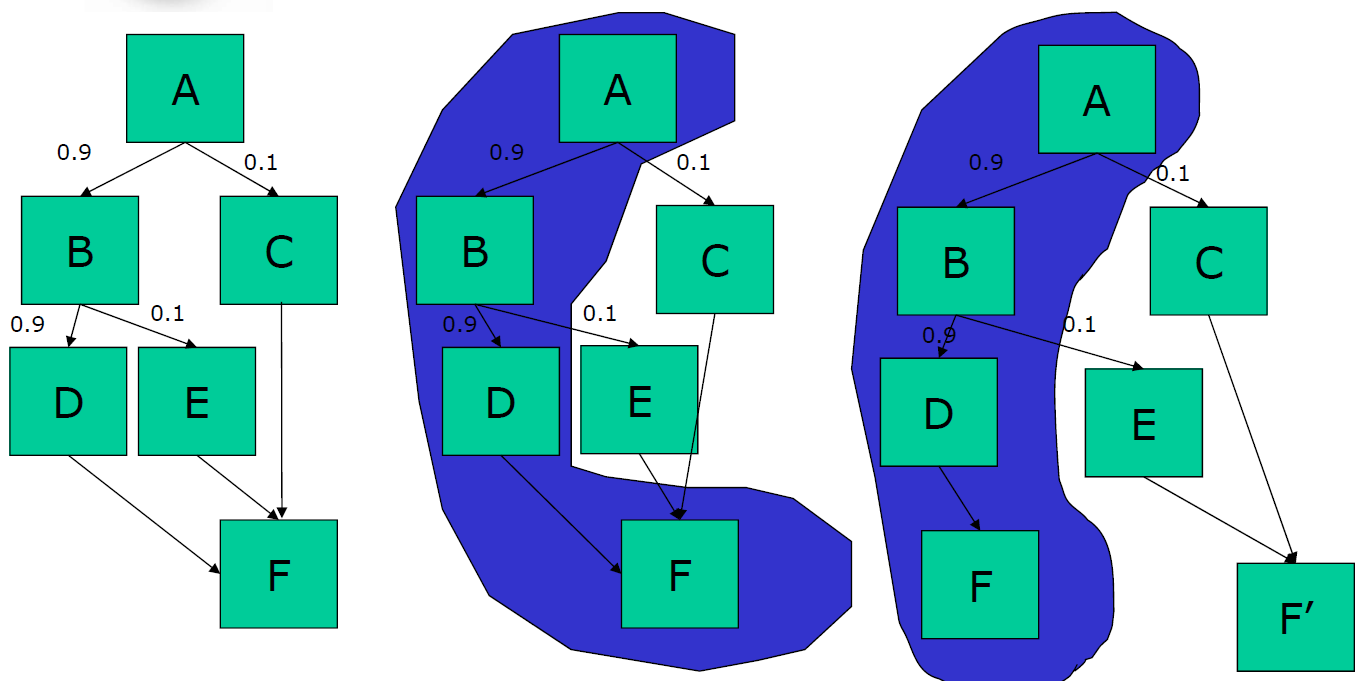
\includegraphics[scale=0.5]{img/superblock.png}
\caption{Realizzazione di un superblocco}\label{fig:superblock}
\end{figure}
\paragraph{Hardware support}
Tutte le tecniche viste fino ad ora si applicano quando il comportamento dei salti è molto predicibile altrimenti il controllo delle dipendenze limita di molto il parallelismo. Per aggirare questo problema possiamo estendere il set di istruzioni per includere delle istruzioni condizionali; utilizzare la speculazione del compilatore con il supporto dell'hardware per permettere di creare codice speculativo mantenendo il comportamento delle eccezioni.\\
Un esempio è \emph{l'esecuzione condizionale} che utilizza un particolare tipo di istruzione come quella seguente:
\begin{verbatim}
(p)		op Rd, R1, R2
\end{verbatim}
dove \texttt{p} è un predicato booleano che condiziona l'operazione \texttt{op}, infatti, \texttt{op} viene \emph{committata} soltanto se \emph{p} risulta \emph{vera}.\\
Avendo effettuato queste modifiche possiamo a questo punto modificare il codice tramite delle \emph{if-conversion} che trasformano i salti in sequenze di istruzioni condizionali e le dipendenze di controllo si trasformano in dipendenze sui dati eliminando così i salti. I vantaggi sono l'eliminazione dei problemi di \emph{miss-prediction} e l'aumento delle dimensione dei basic block. Questa soluzione diventa efficente se le predizione errate e quindi la loro penalità è considerevole e se i salti sono sbilanciati e la parte eseguita più frequentemente è quella più lunga.
